\section{Цель работы}
	Изучить принципы построения нейронных сетей и получить навыки  работы с пакетом прикладных программ Neural Network Toolbox в программной среде MATLAB.
\section{Порядок выполенения работы}
	\subsection{Задача}
		Создать и обучить нейронную сеть с прямым распространением сигнала и обратным  распространением ошибки для вычисления функции
		\[0.1x^2-x\ln{x}, x\in{[1;2]}.\]
		
		Сеть должна состоять, как минимум из 2-х слоёв, и в каждом слое не менее 3-х нейронов. Точность обучения 5\% (не более 1000 эпох).
		
		
	\subsection{Подготовка данных для обучения}
		В качестве входных данных используем значения функции в точках $ x = 1;1.1;...;2 $, т.е. $ N=11 $ значений. 
		
		\begin{ListingEnv}[H]
			\caption{Формирование входных данных}
			% далее метка для ссылки:
			\label{list:hwbeauty}
			% окружение учитывает пробелы и табляции и приеняет их в сответсвии с настройкми
			\begin{lstlisting}[language={Matlab}]
			f(x) = 0.1 * x^2 - x * log(x);
			n=1;
			for i=1.0:+0.1:2.0
				Input(n)=i;
				A(n)= eval( f(i) );
				n=n+1;
			end
			\end{lstlisting}
		\end{ListingEnv}%
	
	\subsection{Создание сети}
		Для решения поставленной задачи формируется трехслойная сеть обратного распространения, включающая 1 нейрон во входном слое с передаточной функцией \textit{logsig} (сигмоидная (логистическая) функция активации), 5 нейронов во втором слое с функцией активизации \textit{logsig} и 1 нейрона в выходном слое с передаточной функцией \textit{purelin} (линейная функция активации). Функция активации вычисляет выход слоя по его входу.
		
		При этом в качестве обучающего алгоритма выбран алгоритм Левенберга-Маркара (Levenberg-Marquardt - \textit{trainlm}). Этот алгоритм обеспечивает быстрое обучение, но требует много ресурсов. Но существуют и другие алгоритмы (\textit{trainbfg}, \textit{trainrp}, \textit{trainscg}, и др.). По умолчанию используется \textit{trainlm}. Указанная сеть формируется с помощью процедуры:
		
		\begin{ListingEnv}[H]
			\caption{Создание сети}
			% далее метка для ссылки:
			\label{list:hwbeauty}
			% окружение учитывает пробелы и табляции и приеняет их в сответсвии с настройкми
			\begin{lstlisting}[language={Matlab}]
			net=newff(minmax(Input),[1,5,1],{'logsig' 'logsig' 'purelin'},'trainlm');
			\end{lstlisting}
		\end{ListingEnv}%
	
	\subsection{Обучение сети}
		Задается функция оценки функционирования \textit{sse}. В этом случае в качестве оценки вычисляется сумма квадратичных отклонений выходов сети от эталонов. Затем задается критерий окончания обучения – значение отклонения, при котором обучение будет считаться законченным. После задается максимальное количество циклов обучения. После того, как будет выполнено это количество циклов, обучение будет завершено, и, наконец, начинается обучение:
		
		\begin{ListingEnv}[H]
			\caption{Обучение сети}
			% далее метка для ссылки:
			\label{list:hwbeauty}
			% окружение учитывает пробелы и табляции и приеняет их в сответсвии с настройкми
			\begin{lstlisting}[language={Matlab}]
			net.performFcn='sse';
			net.trainParam.goal=0.01;
			net.trainParam.epochs=1000;
			[net,tr] = train(net,Input,A);
			
			plotperform(tr);
			\end{lstlisting}
		\end{ListingEnv}%
	
		Процесс обучения иллюстрируется графиком зависимости оценки функционирования от номера цикла обучения:
		
		\begin{figure}[ht!] 
			\center
			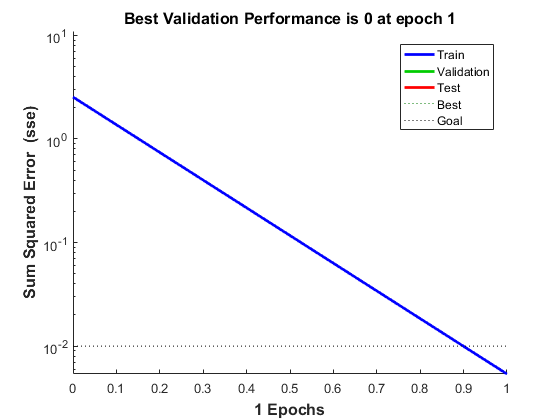
\includegraphics [width=\textwidth] {training}
			\caption{Зависимость оценки от цикла обучения} 
		\end{figure}
		\FloatBarrier
		
	\section{Тестирование}
		Исследуем степень достоверности результатов вычислений сети на тестовом массиве входных данных. В качестве тестового массива необходимо использовать массив, компоненты которого отличаются от компонентов массива, использованного для обучения.
		
		Для оценки достоверности результатов работы сети можно воспользоваться результатами регрессионного анализа, полученными при сравнении эталонных значений со значениями, полученными на выходе сети, когда на вход поданы входные векторы тестового массива.
		
			\begin{ListingEnv}[H]
			\caption{Формирование тестового массива и тестирование.}
			% далее метка для ссылки:
			\label{list:hwbeauty}
			% окружение учитывает пробелы и табляции и приеняет их в сответсвии с настройкми
			\begin{lstlisting}[language={Matlab}]
			n=1;
			for i=1.0:+0.01:2.0
				TestInput(n)=i;
				B(n)= eval( f(i) );
				n=n+1;
			end
			
			Y=sim(net,TestInput);
			postreg(Y,B);
			\end{lstlisting}
		\end{ListingEnv}%
	
		\begin{figure}[ht!] 
			\center
			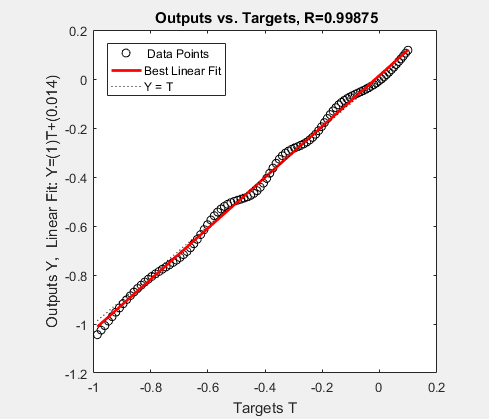
\includegraphics [width=\textwidth] {test}
			\caption{Сравнение результата симуляции с фактическими значениями функции.} 
		\end{figure}
		\FloatBarrier